% The network architecture is summarized in Figure~\ref{fig:arch}. The method follows the traditional format of a convolutional neural network, with one convolutional, batch normalization, and max pooling layer, followed by two fully connected layers. The chosen architecture possesses three notable considerations.  We elaborate upon these considerations below.
We learn a metric by learning to embed time series into a vector space and comparing the resulting vectors with the Euclidean distance. Our embedding function is takes the form of a convolutional neural network, shown in Figure~\ref{fig:arch}. The architecture rests on three basic layers: a convolutional layer, maxpooling layer, and a fully connected layer.

The convolutional layer is included to learn the appropriate subsequences from the input. The network employs one-dimensional filters convolved over all time steps, in contrast to traditional two-dimensional filters used with images. We opt for one-dimensional filters because time series data is characterized by infrequent sampling. Convolving over each of the variables at a given timestep has little intuitive meaning in developing an embedding when each step measurement has no coherent connection to time.  For discussion regarding the mathematical connection between a learned convolutional filter and traditional subsequence-based analysis of time series, we direct the reader to \citep{cui2016multi}.

The maxpooling layer allows the network to be resilient to translational noise in the input time series. Unlike most existing neural network architectures, the windows over which we max pool are defined as percentages of the input length, not as constants. This level of pooling allows us to heavily downsample and denoise the input signal and is fed into the final fully connected layer.

We downsample heavily after the filters are applied such that each time series is reduced to a fixed size. We do so primarily for efficiency---further discussion on parameter choice for Jiffy may be found in Section 6.

We then train the network by appending a softmax layer and using cross-entropy loss with the ADAM \citep{adam} optimizer. We experimented with more traditional metric learning loss functions, rather than a classification objective, but found that they made little or no difference while adding to the complexity of the training procedure; specific loss functions tested include several variations of Siamese networks \citep{siameseOrig,siameseRecurrent} and the triplet loss \citep{tripletMetric}. % The unsupervised network swaps the classification loss function and softmax layer for the reconstruction loss of an autoencoder. The unsupervised model is trained on a squared reconstruction loss objective function.


% We optimize our model using ADAM \citep{adam} During training time, we batch normalize after the convolutional layer.

% \vspace{8mm}

% ------------------------------------------------
\subsection{Complexity analysis}
% ------------------------------------------------

For ease of comparison to more traditional distance measures, such as DTW, we present an analysis of Jiffy's complexity.

Let $T$ be the length of the $D$-variable time series being embedded, let $F$ be the number of length $K$ filters used in the convolutional layer, and Let $L$ be the size of the final embedding.
The time to apply the convolution and ReLU operations is $\Theta(TDFK)$. Following the convolutional layer, the maxpooling and downsampling require $\Theta(T^2DF)$ time if implemented naively, but $\Theta(TDF)$ if an intelligent sliding max function is used, such as that of \citep{lemireMax}. Finally, the fully connected layer, which constitutes the embedding, requires $\Theta(TDFL)$ time.

The total time to generate the embedding is therefore $\Theta(TDF(K + L))$. Given the embeddings, computing the distance between two time series requires $\Theta(L)$ time. Note that $T$ no longer appears in either expression thanks to the max pooling.

With $F = 16$, $K = 5$, $L = 40$, this computation is dominated by the fully connected layer. Consequently, when $L \ll T$ and embeddings can be generated ahead of time, this enables a significant speedup compared to operating on the original data. Such a situation would arise, e.g., when performing a similarity search between a new query and a fixed or slow-changing database \citep{bolt}. When both embeddings must be computed on-the-fly, our method is likely to be slower than DTW and other traditional approaches. % faster than RNN-based embeddings, but % When $T < DF(K + L) = 720$,

\begin{figure*}[h]
\begin{center}
% 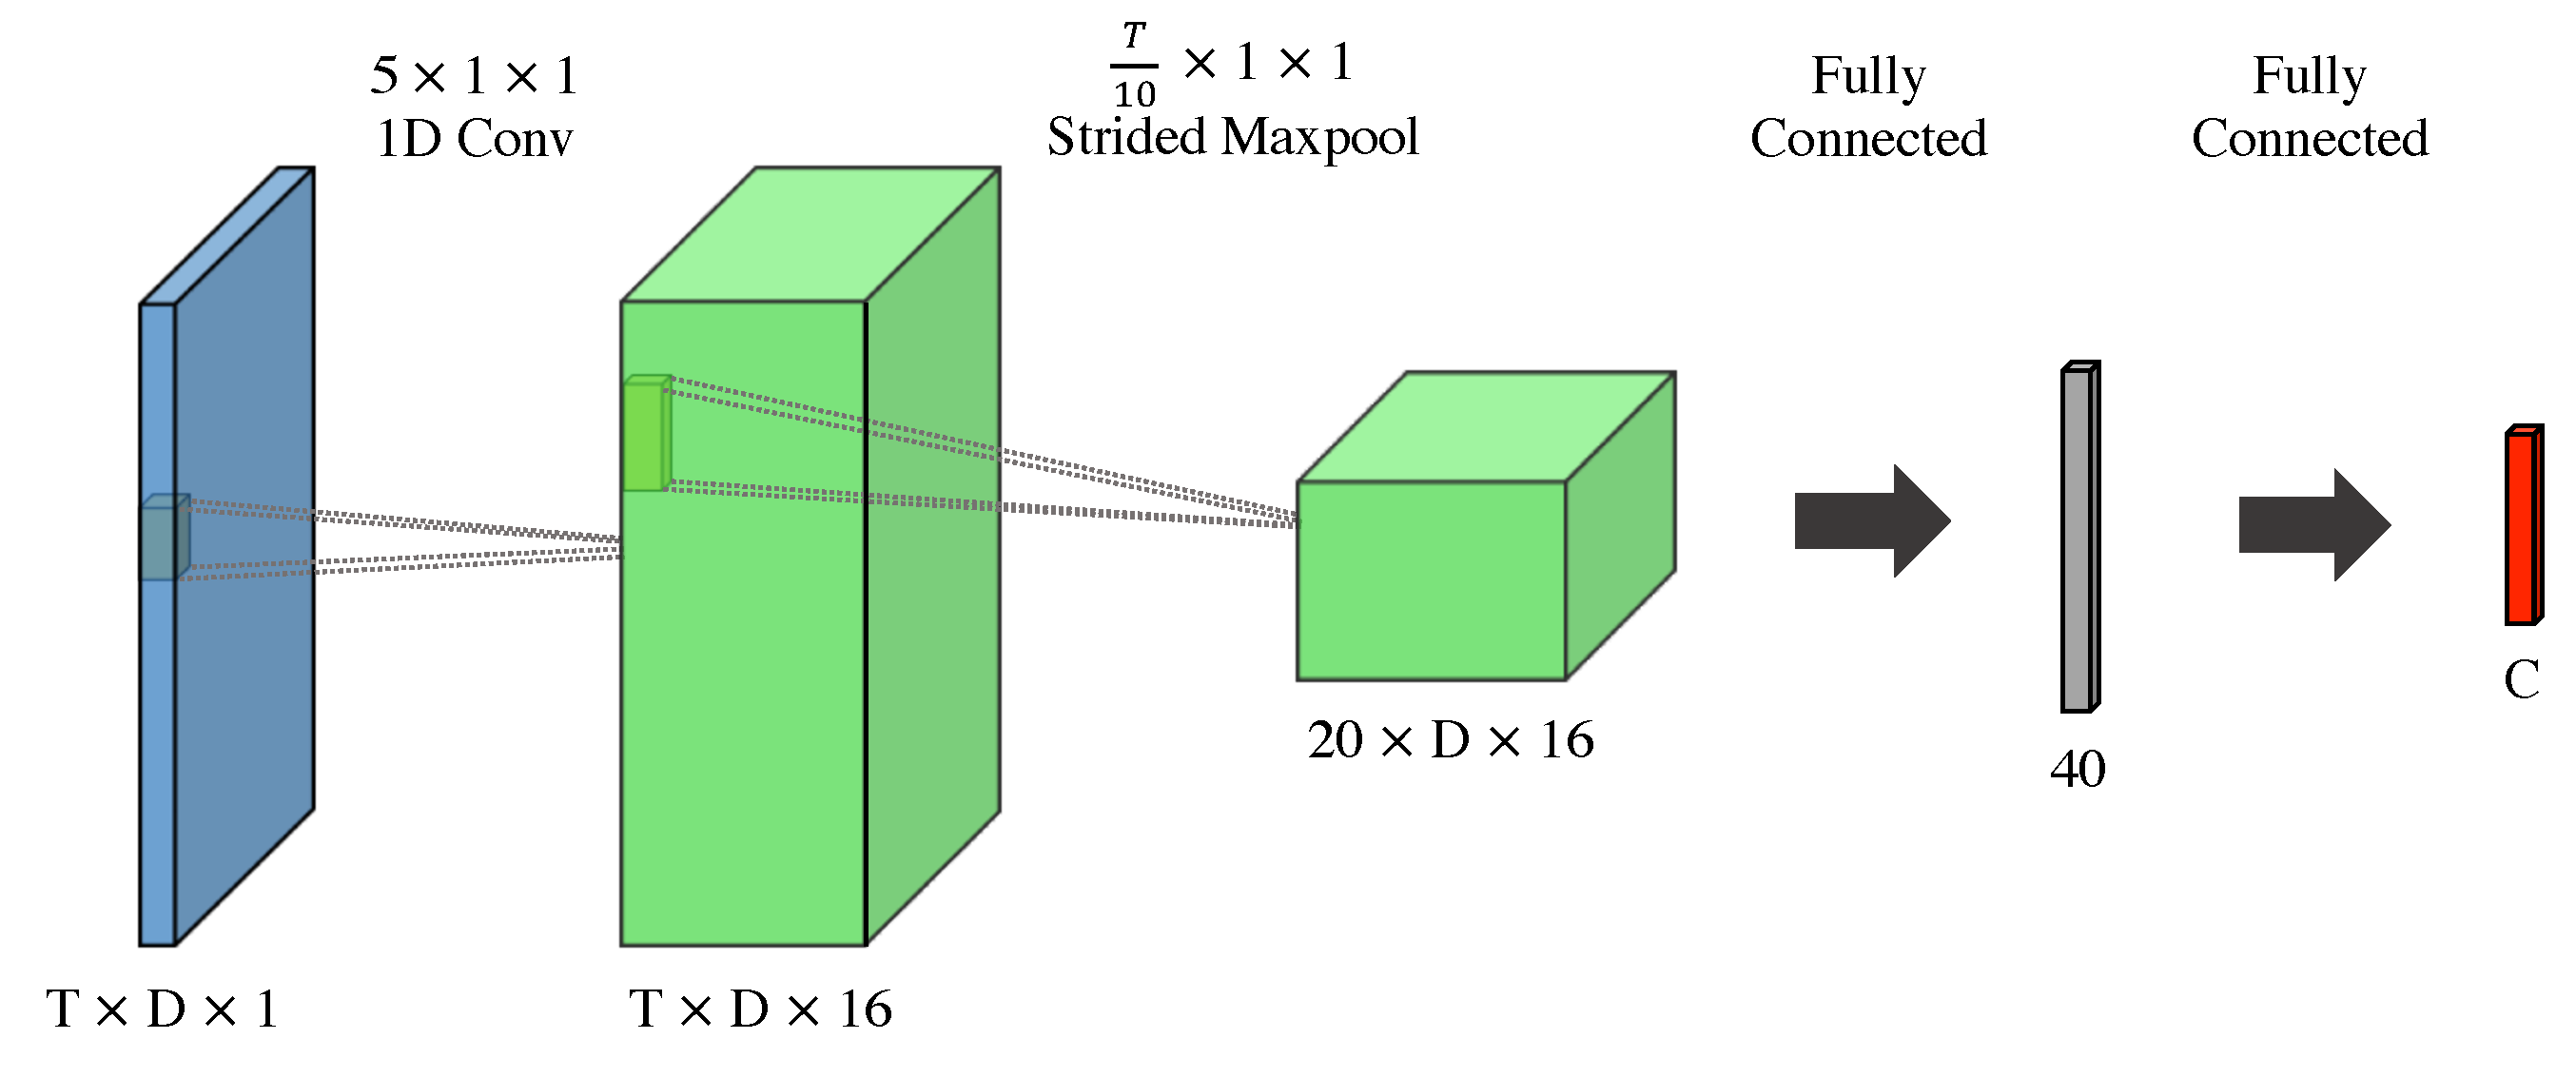
\includegraphics[width=\linewidth]{arch}
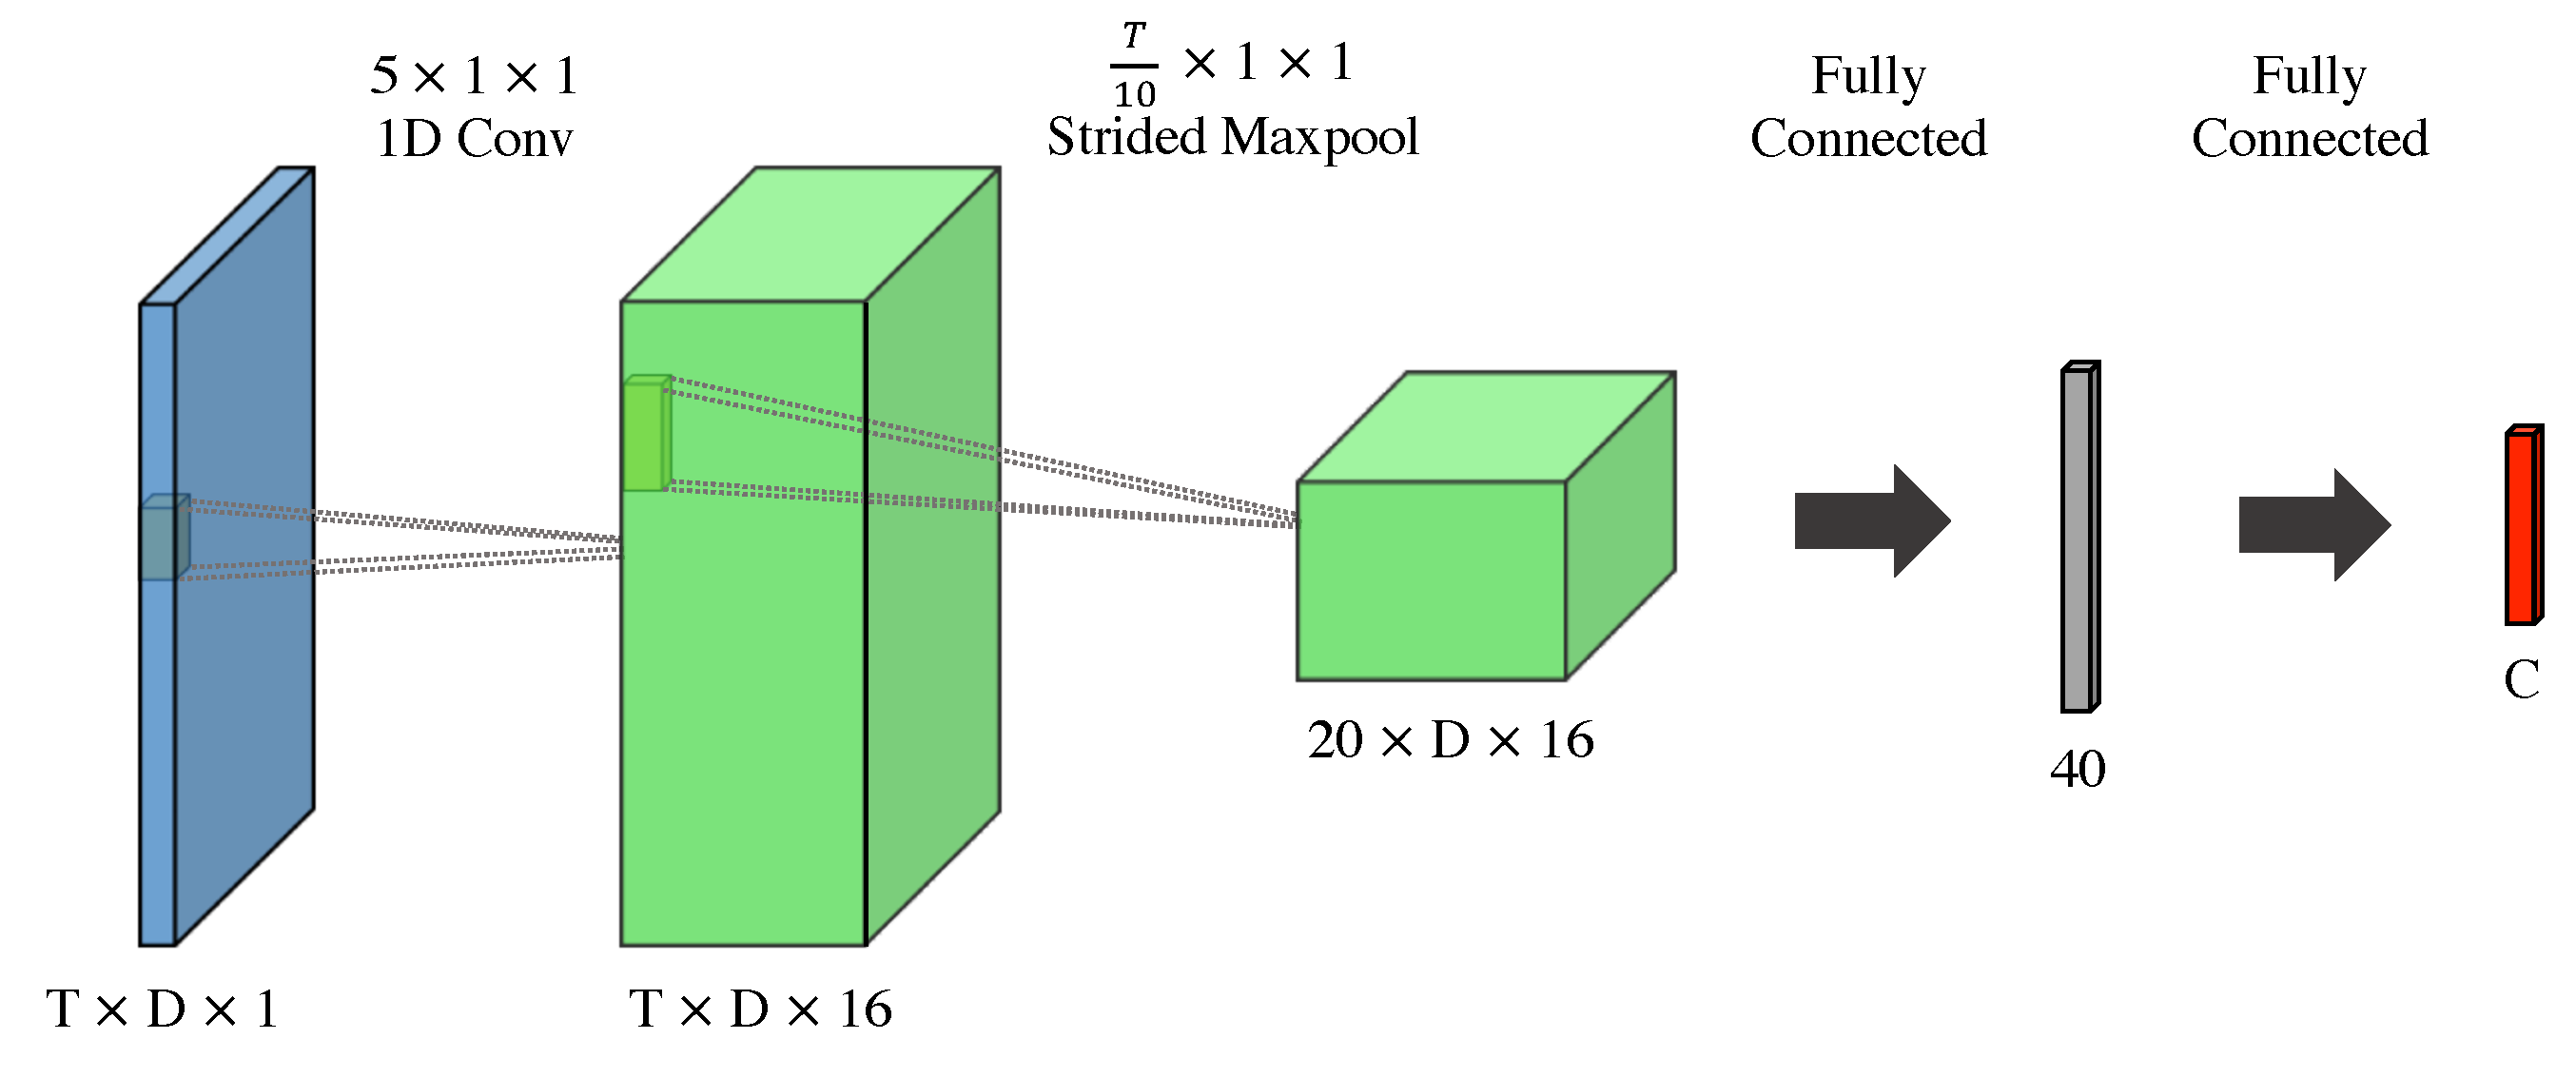
\includegraphics[width=.9\textwidth]{arch}
% \vspace*{-2mm}
\caption{Architecture of the proposed model. A single convolutional layer extracts local features from the input, which a strided maxpool layer reduces to a fixed-size vector. A fully connected layer with ReLU activation carries out further, nonlinear dimensionality reduction to yield the embedding. A softmax layer is added at training time.}
\label{fig:arch}
\end{center}
\end{figure*}
%\vspace{8m}

% \subsubsection{Bag-of-Patterns}

% Several recent representation approaches describe a time series as a set of counts detailing how many times each ``pattern'' from some fixed set takes place within it. Common patterns used include being the preimage of particular SAX words \citep{saxVSM}, or containing particular frequency content \citep{boss, weasel}.

% Our method can be seen as a continuous, trainable, relaxation of this model. First, observe that each convolutional neuron with ReLU activation can be cast as a detector for a particular pattern; when the pattern is not present, the neuron's output is 0; when it is present, the neuron's output is a continuous, rather than binary, representation of how ``present'' it is. This neuron cannot necessarily represent the exact patterns used by other methods, but if they are based on frequency content, it .

% -Suppose that each filter describes the presence of one pattern. Then if each neuron in the first fully connected layer listens to one feature map with weights tied at 1, it's just counting the number of times that pattern happens; first FC layer is then a histogram. Also note that this requires having no max pooling...


% -The first paper

% \subsubsection{Frequency-domain binning}

% Frequency-domain binning vs convolutional layers

% like shapelet stuff, but with MLP on shapelet repr, not decision tree or SVM

% // People don't seem to realize this and it's bothering me. I need to write this.



% -if one removes our fully connected layers (and adds in some additional machinery for differentiating with respect to filter length), one effectively recovers the shapelet learning algorithm of \citep{learningShapelets}. Moreover, if one further requires the shapelets to be drawn from the finite set of length $M$ subsequences observed in the data, one recovers the objective of most previous shapelet learning work.

% This can equivalently be rewritten as:
% \begin{align}
% 	\min_n \norm{\x^n - \s}^2 &= \min_n \norm{\x^n}^2 + \norm{\s}^2 - 2 \s \cdot \x^n \\
%     &= \norm{s}^2 - \frac{1}{2}\max_n \s \cdot \x^n - \norm{\x^n}^2
% %     &= b + a \max_n \s \cdot \x^n - \norm{\x^n}^2
% %     &= b + a \max_n x \ast s - \norm{\x^n}^2
% \end{align}

% \begin{align}
% 	\delta(\x, \s) \triangleq \min_n \sum_{i = 1}^{M} (x_{n - 1 + i} - s_{i})^2, M-1 < n \le N
% \end{align}
% With mean normalization, we obtain the slightly more complex:
% \begin{align}
% % \begin{split}
% 	\delta(\x, \s) \triangleq \min_n \sum_{i = 1}^{M} ( (x_{n - 1 + i} - \bar{x}_n) -
%     (s_{i} - \bar{s}) ) ^2
% % \end{split}
% \end{align}
% where
% \begin{align}
% 	\bar{s} &\triangleq \frac{1}{M} \sum_{i = 1}^{M} s_i \\
%     \bar{x}_n &\triangleq \frac{1}{M} \sum_{i = n - M + 1}^{n} x_i
% \end{align}
% Letting $\omega$ to be a vector of $M$ ones, this can be rewritten as:
% \begin{align}
% 	\delta(\x, \s) \triangleq \min_n \sum_{i = 1}^{M} ( (x_{n - 1 + i} - \bar{x}_n) -
%     (s_{i} - \bar{s}) ) ^2
% \end{align}


% \begin{align}
% % \begin{split}
% 	\delta(\x, \s) \triangleq \min_n \sum_{i = 1}^{m} \bigg( \frac{(x_{n - 1 + i} - \bar{x}_n}{\sigma_{x,n}} -
%     \frac{s_{i} - \bar{s}}{\sigma_s} \bigg) ^2
% % \end{split}
% \end{align}
% where
% \begin{align}
% 	\bar{s} &\triangleq \frac{1}{m} \sum_{i = 1}^{m} s_i \\
%     \bar{x}_n &\triangleq \frac{1}{m} \sum_{i = n - m + 1}^{n} x_i \\
%     \sigma_{x,n} &\triangleq \sqrt{ \frac{1}{m} \sum_{i = n - m + 1}^{n} (x_i - \bar{x}_n)^2}
% \end{align}


% Let $\vec{x}$ be a univariate time series and let $\s$ be a length $M$ vector. Ignoring the initial $m-1$ time steps, the convolution of $\x$ and $\s$, $\x \ast \s$, can be defined as:
% \begin{align}
% 	(\x \ast \y)(n) \triangleq \sum_{i = n-m+1}^{n} x_n y_{m - i + 1}
% \end{align}
% Suppose now that instead of treating $\vec{s}$ as a filter, we treat it as a shapelet.


% Get to here:


% -Euclidean distances are just convolving, but then negating and adding some squared norms
% -With z-normed euclidean distances, we're subtracting off output from a boxcar filter, and dividing by output from a boxcar filter over square of the time series
% 	-and also constraining the filters to live on unit hypersphere in Euclidean space
% -and biggest constraint is of course that people typically only allow shapelets that
% -shapelets max pool over whole ts, but we allow max pooling over only part of it
% -and shapelets use cross-corr, not convolution, so order is reversed

% -if one removes our fully connected layers (and adds in some additional machinery for differentiating with respect to filter length), one effectively recovers the shapelet learning algorithm of \citep{learningShapelets}. Moreover, if one further requires the shapelets to be drawn from the finite set of length $M$ subsequences observed in the data, one recovers the objective of most previous shapelet learning work.
% -fully connected layers basically mean MLP instead of linear model or decision tree on top of shapelet repr
